\documentclass[12pt]{article}

\usepackage[a4paper,margin=2.5cm]{geometry}
\usepackage[spanish,es-tabla]{babel}
\usepackage[utf8]{inputenc}
\usepackage[T1]{fontenc}
\usepackage{amsmath}
\usepackage{amssymb}
\usepackage{graphicx}
\usepackage{float}
\usepackage{booktabs}
\usepackage{hyperref}

\hypersetup{
    colorlinks=true,
    linkcolor=black,
    urlcolor=blue
}

\setlength{\parindent}{0pt}
\setlength{\parskip}{0.75em}

\newcommand{\horrule}[1]{\rule{\linewidth}{#1}}

\title{
    
\includegraphics[width=6.5cm]{Fig/usm.png}\\[0.4cm]
    \normalfont\normalsize
    Universidad Técnica Federico Santa María, Departamento de Informática\\[0.4cm]
    \horrule{0.5pt}\\[0.35cm]
    \huge\textbf{Tarea 1: Arreglo de Filtros de Bayer e Interpolación (Demosaicking)}\\[-0.1cm]
    \horrule{2pt}\\[0.25cm]
}

\author{Profesor Dr. Nelson Díaz, \href{mailto:nelson.diazd@usm.cl}{nelson.diazd@usm.cl}, F-311}
\date{7 de agosto de 2026}

\begin{document}

\maketitle

El informe de tarea debe entregarse el día 19 de Agosto de 2026, en éste deben resolver los ejercicios que se presentan en la guía en forma de informe, además anexar los archivos que generen, por ejemplo \texttt{.py}, \texttt{.ipynb}, \texttt{.mat}, \texttt{.m}, \texttt{.fig}, etc. En el informe deben describir brevemente los experimentos realizados, incluyendo las secciones de: resumen, descripción de experimentos y conclusiones, se sugiere elaborar el informe en \LaTeX{} para facilitar la escritura de ecuaciones. Enviar una carpeta comprimida con los archivos al correo electrónico: \href{mailto:nelson.diazd@usm.cl}{nelson.diazd@usm.cl}, con el asunto \textbf{Tarea -- 1-Fotografía computacional} y el nombre de la carpeta comprimida \textbf{Lab--NombreApellido}, donde Nombre es su primer nombre y Apellido es su primer apellido.

\textbf{Precaución:} cualquier intento de copia o fraude anula el laboratorio y hace merecedor de cero en la nota del laboratorio que se esté desarrollando.

\section{Objetivo de aprendizaje}

Identificar los filtros que componen un arreglo de filtros Bayer y resolver la tarea de interpolación, más conocida en fotografía computacional como \textit{demosaicking}, con algoritmos de interpolación del estado del arte. Al terminar esta tarea el estudiante será capaz de simular un sistema de fotografía de color y reconstruir la imagen de color.

\section{Introducción}

La fotografía en color se compone de dos etapas: una de muestreo de la señal que genera un mosaico mediante un arreglo de filtro Bayer, también conocido como filtro de color, y una etapa computacional que implica un algoritmo de reconstrucción.

\subsection{Arreglo de filtros de Color}

El arreglo de filtro Bayer es una matriz con tres filtros espectrales de banda ancha correspondientes a las longitudes de onda del rojo, verde y azul, ver Figura~\ref{fig:bayer}. Sea $T_c = \mathbf{1} \otimes B_c$, donde $\otimes$ indica producto Kronecker entre dos matrices, $c \in \{0,1,2\}$ indican los tres canales rojo, verde y azul, $\mathbf{1} \in \{1\}^{\frac{N}{2} \times \frac{N}{2}}$ es una matriz de solo unos, y $B_c \in \{0,1\}^{2 \times 2}$.

\begin{figure}[H]
    \centering
    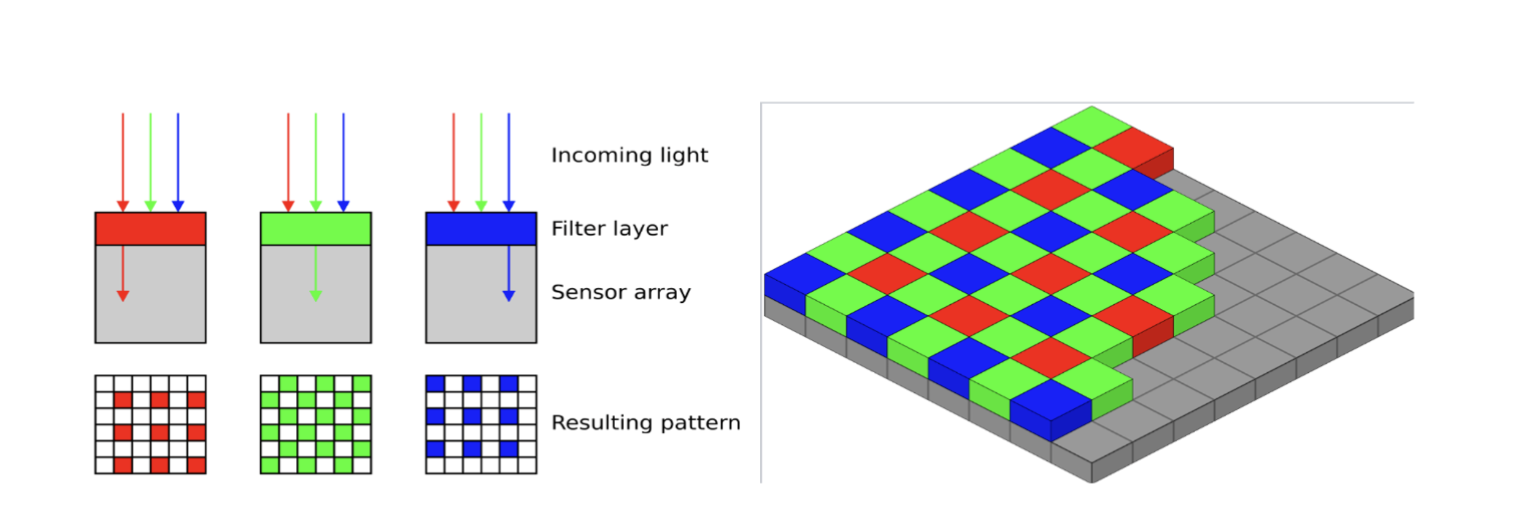
\includegraphics[width=0.85\linewidth]{Fig/fig1.png}
    \caption{El arreglo de filtros Bayer se compone de tres filtros: rojo, verde, azul, que crean un mosaico del campo de luz incidente.}
    \label{fig:bayer}
\end{figure}

\[
B_0 =
\begin{bmatrix}
1 & 0 \\
0 & 0
\end{bmatrix},
\qquad
B_1 =
\begin{bmatrix}
0 & 1 \\
1 & 0
\end{bmatrix},
\qquad
B_2 =
\begin{bmatrix}
0 & 0 \\
0 & 1
\end{bmatrix}.
\]

\subsection{Modelo de Medición}

El modelo de medición submuestrea cada canal $I_c$ de acuerdo a las longitudes de onda de cada filtro $T_c \in \mathbb{R}^{N \times N \times C}$, obteniendo un mosaico

\begin{equation}
Y = \sum_{c=1}^{C} T_c \odot I_c,
\end{equation}

donde $Y \in \mathbb{R}^{N \times N}$, siendo $N^2$ el número total de píxeles de la cámara y donde los tensores $I \in \mathbb{R}^{N \times N \times C}$ y $T \in \{0,1\}^{N \times N \times C}$ corresponden al campo incidente y tensor binario del filtro Bayer y $C$ es el número de canales, es decir, 3 canales.

\subsection{Interpolación 2D o Demosaicking}

El proceso de recuperación empieza generando un tensor con las muestras y los valores no capturados:

\begin{equation}
\bar{I}_c = T_c \odot Y.
\end{equation}

Luego, para recuperar la imagen de color a partir del mosaico se realiza un filtrado por convolución entre el tensor de las muestras $\bar{I}$ y el filtro $H$ en cada canal.

\begin{equation}
\hat{I}_c = \bar{I}_c * H_c,
\end{equation}

donde $*$ denota convolución, donde $\hat{I}$ es la imagen RGB recuperada.

\section{Ejercicios}

\begin{itemize}
    \item Implementar un sistema de fotografía computacional de color en Python, usando el filtro Bayer visto en clase para generar el mosaico o medida \textit{Bayer Filter}; seleccionar algoritmos de interpolación 2D, por ejemplo, interpolación bicúbica, que le permitan interpolar cada uno de los canales.

    \item Para la tarea 1 usar todo el dataset Kodak que se compone de 24 imágenes RGB, ver Figura~\ref{fig:kodak}.

    \item Usar métricas de calidad espacial como el \textit{Peak-Signal-to-Noise Ratio} (PSNR), \textit{Structural Similarity Index} (SSIM) y \textit{Spectral Angle Mapper} (SAM) para medir la calidad espectral.
\end{itemize}

\begin{figure}[H]
    \centering
    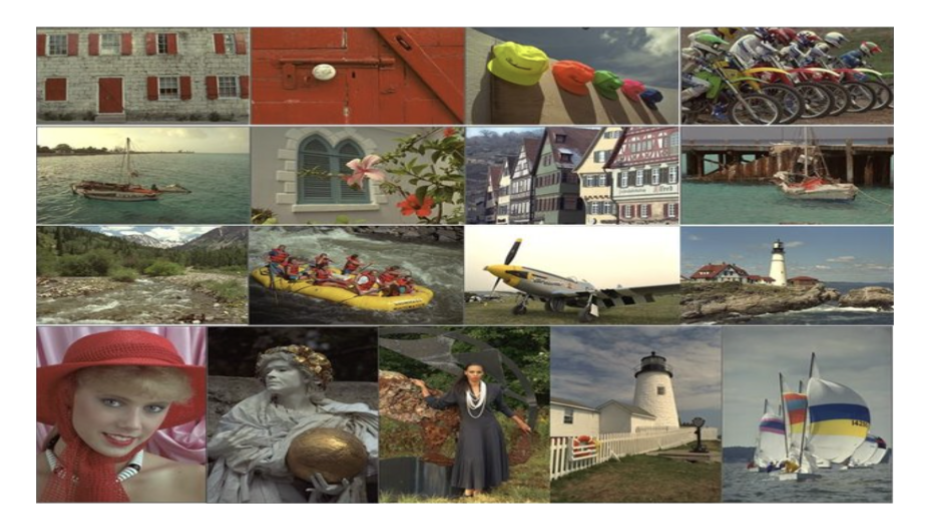
\includegraphics[width=0.85\linewidth]{Fig/fig2.png}
    \caption{El dataset Kodak está compuesto por 24 imágenes; a continuación se presentan algunas.}
    \label{fig:kodak}
\end{figure}

La proporción de señal a ruido o \textit{Peak Signal-to-Noise Ratio} (PSNR) en decibelios (dB) está dada por:

\begin{equation}
\mathrm{PSNR} = 10 \cdot \log_{10}\left(\frac{\mathrm{MAX}_I^2}{\mathrm{MSE}}\right),
\end{equation}

donde $\mathrm{MAX}_I$ representa el máximo valor posible para el píxel de la imagen, por ejemplo 255 para una imagen de 8 bits.

El error cuadrático medio está dado por:

\begin{equation}
\mathrm{MSE} =
\frac{1}{m \cdot n}
\sum_{i=0}^{m-1}
\sum_{j=0}^{n-1}
\left[I(i,j)-K(i,j)\right]^2.
\end{equation}

El índice de similitud estructural se define como:

\begin{equation}
\mathrm{SSIM}(x,y) =
\frac{(2\mu_x\mu_y + C_1)(2\sigma_{xy} + C_2)}
{(\mu_x^2 + \mu_y^2 + C_1)(\sigma_x^2 + \sigma_y^2 + C_2)}.
\end{equation}

Donde:

\begin{itemize}
    \item $\mu_x$ y $\mu_y$ son las medias locales, o promedios de luminancia, de $x$ e $y$.
    \item $\sigma_x^2$ y $\sigma_y^2$ son las varianzas locales, o contraste, de $x$ e $y$.
    \item $\sigma_{xy}$ es la covarianza local, o similitud estructural, de $x$ e $y$.
    \item $C_1 = (K_1L)^2$ y $C_2 = (K_2L)^2$ son constantes estabilizadoras.
    \item $L$ es el rango dinámico de los valores de los píxeles, típicamente $2^B - 1$, donde $B$ son bits por píxel.
    \item $K_1 \ll 1$ y $K_2 \ll 1$ son pequeñas constantes escalares.
\end{itemize}

El ángulo espectral se calcula como:

\begin{equation}
\theta =
\arccos
\left(
\frac{\sum_{i=1}^{n} T_iR_i}
{\sqrt{\sum_{i=1}^{n} T_i^2}\sqrt{\sum_{i=1}^{n} R_i^2}}
\right).
\end{equation}

Donde:

\begin{itemize}
    \item $\theta$ es el ángulo espectral, generalmente medido en radianes.
    \item $n$ representa el número total de bandas espectrales.
    \item $T_i$ es el valor del espectro de prueba/píxel en la banda $i$.
    \item $R_i$ es el valor del espectro de referencia/componente extremo en la banda $i$.
\end{itemize}

\begin{center}
\begin{tabular}{ccc}
\toprule
PSNR & SSIM & SAM \\
\bottomrule
\end{tabular}
\end{center}

Note que al usar algoritmos simples producen artefactos como difuminación, el efecto de cremallera y falso color, ver Figura~\ref{fig:artefactos}.

\begin{figure}[H]
    \centering
    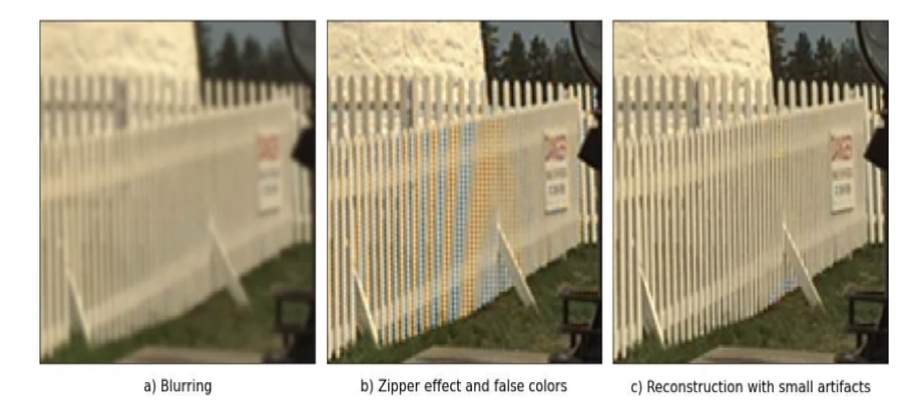
\includegraphics[width=0.85\linewidth]{Fig/fig3.png}
    \caption{Artefactos: (a) difuminado, (b) efectos cremallera y falso color, (c) reconstrucción con artefactos.}
    \label{fig:artefactos}
\end{figure}

Tabular las métricas de calidad para cada imagen y el promedio y la desviación estándar para todo el dataset.

\textbf{Bonus:} implementar este algoritmo de demosaicking paper.

\end{document}
